\chapter{Implementation details}
\label{sec:additional-algs}

This chapter sums up some information about the implementation. We explain why we chose C++ and Python to implement the project and present some central algorithms that were developed during this project.

\section{Choice or programming language(s)}
\label{sec:implementation-prog-lang}

The first question we faced was the programming language to use. We first tried to develop a prototype with Maple, because Maple already supports many mathematical concepts (in particular graph theory and probability theory) that might later be useful.

However, we quickly realized that probably Maple has some downsides for this use case: We needed something that was able to cope with quite large amount of data. While Maple might be able to do so if you are experienced enough, we went for C++, sacrificing the elegant notation of Maple, but gaining speed and control over how data are organized in memory. We also considered simple C, but quickly discarded it, because we did not want to implement some basic data structures ourselves, but instead relied on well-tested implementations (especially of Maps and Vectors). As a bonus, there are many good C++ libraries out there, some of which we made use of (Boost and GMP).

Additionally, we looked a simple language to solve several non-critical one-time tasks, such as e.g. generating a database containing all (distinct) intrees or some data analysis. We chose Python.

\section{General structure}
\label{sec:implementation-general-structure}

The developed program basically starts off given a single intree, a certain number of processors and a scheduling strategy. According to this strategy, we then compute all initial combinations of scheduled tasks, i.e. all initial snapshots (up to equivalent snapshots).

Starting at an initial snapshot, we then recursively compute all its successors, i.e. we simulate which task finishes first and wich task shall be chosen next according to the given scheduling strategy. All of these events (task finishes, next task is chosen) are associated with a certain probability. We do this until we reach the intree containing only 1 task, which then denotes the end of the scheduling process. We thereby eliminate equivalent snapshots in order to save memory.\footnote{We also implemented a variant that does not eliminate equivalent snapshots. However, this variant quickly became too slow as the number of tasks increased.}

After the whole snapshot DAG has been computed we can compute the expected run times of the initial snapshots (recursively, as explained in section \ref{sec:introduction-compute-expected-time-schedule}).

Moreover, the program is capable of ``excluding the scheduler's bad choices'', i.e. it determines where the scheduler has chosen a good and where it has chosen a bad task. Then, the program discards the bad choices and leaves only the good choices, yielding a (possibly) new schedule that is optimal for a given intree.

In order to keep the program fast, we thereby had to cache quite a lot of results (since the recursions through the snapshot DAG would otherwise requiring computing the same things over and over). This, of course, leads to increased memory consumption.

We implemented support for various representation of probabilities and expected run times, most notably floating point numbers. Other possible representation include doubles or rationals (through the use of e.g. the GNU Multiple Precision library).

\section{Representation of intrees and snapshots}
\label{sec:implementation-repr-intrees-snapshots}

For the representation of intrees and snapshots, we tried to find a good balance between ease of use, memory consumption and speed. We thereby rely on well-tested data structures from the C++ standard library. We now describe on a very high level how we implemented the needed data structures.

Intrees are basically maintained as a collection of edges that -- implicitly -- also store the vertices resp. tasks. We store the edges in an array such that an edge $(i,j)$ is stored as $array[i]=j$, i.e. the start of the edge is used as the array index while the target of the edge is used as the element at that particular position in the array. This is possible since we are dealing with intrees only and enables a quick lookup on which task is a successor of a given task.

Snapshots store the following things:
\begin{itemize}
\item The corresponding intree (in normalized form -- see section \ref{sec:algorithm-equivalent-snapshot}).
\item The set of currently scheduled tasks.
\item The set of its successors in the snapshot DAG and the corresponding transition probability.
\end{itemize}

Additionally, we cache many results that are frequently needed and expensive to recompute, such as the expected run time. In order to be able to reuse snapshots so that we do not recompute results for equivalent snapshots, we need some data structure that enables us to retrieve an equivalent snapshot if it already has been constructed. Therefore we introduced a pool that manages all snapshots and can be used to avoid duplicates of (equivalent) snapshots.

\newcommand{\treegeq}[1][X]{\stackrel{\text{#1}}{\geq}}

\section{Computing equivalent snapshots}
\label{sec:algorithm-equivalent-snapshot}

As mentioned in section \ref{sec:intro-first-glance-schedules}, it is possible to combine certain snapshots into one single snapshot, thereby avoiding redundant computations. The requirements for two snapshots being equivalent have been discussed there.

It is a notable fact that we can determine in polynomial time (w.r.t. the number of nodes) whether two snapshots are equivalent. This computation involves foremost a check whether the two corresponding intrees are isomorphic. 

%While it seems to be quite hard to check isomorphism for general graphs (\todo{unbedingt Referenz!}), it is feasible for intrees.

While there currently is no known algorithm that checks isomorphism in polynomial time \emph{for general graphs} (see \cite{arora2009computational}), there is a simple algorithm for isomorphism of intrees. The idea behind this algorithm is to recursively sort the predecessors of a task according to the number of their respective predecessors. An early description of this algorithm can be found e.g. in \cite{aho1974design}. We can easily adapt this isomorphism check to our needs in the sense that we can construct an algorithm that constructs a ``canonical snapshot'', and all equivalent snapshots are converted to exactly this canonical snapshot.

One thing to keep in mind is that we have to explicitly take care of the currently scheduled tasks, i.e. we have to adopt the algorithm to distinguish between scheduled and unscheduled tasks.

\subsection{The algorithm}
\label{sec:algorithm-equiv-snapshots-actual-algo}

The algorithm basically relies on an ordering of intrees (there are of course many possible, but we use a simple one).

\begin{definition}[Ordering of intrees with preferred tasks]
  We introduce an ordering denoted by $\treegeq$. For two intrees $I_1$ and $I_2$ and a set $X$ of tasks, we define $I_1 \treegeq I_2$ inductively. 
  \begin{itemize}
  \item If both $I_1$ and $I_2$ consist only of a root, we have $I_1 \treegeq I_2$ if and only if the root of $I_1$ is in $X$ and the root of $I_2$ is not in $X$.
  \item If the root of $I_1$ has less predecessors than the root of $I_2$, then $I_1 \treegeq I_2$.
  \item If the root of $I_1$ has the same number $r$ of predecessors as the root of $I_2$, we sort the corresponding predecessors $p_1,\dots,p_r$ resp. $q_1,\dots,q_r$ (in $I_1$ resp. $I_2$ according to $\treegeq$). Then, if $p_i \treegeq q_i \forall i\in\{1,2,\dots,r \}$, we have $I_1 \treegeq I_2$.
  \end{itemize}
\end{definition}

\todo{Examples!}

The algorithm recursively sorts the tasks in the intree according to the ordering $\treegeq$. It is shown in algorithm \ref{alg:compute-canonical-snapshot}.

\begin{algorithm}
  \begin{algorithmic}
    \Procedure{CanonicalSnapshot}{$s$} \Comment{Returns the canonical snapshot for snapshot $s$}
    \State $t \gets s.intree$ \Comment{Retrieve root of intree}
    \State $X \gets s.scheduled$ \Comment{Retrieve scheduled tasks}
    \State \textbf{return} \Call{CanonicalIntree}{$t, X$} 
    \EndProcedure
    \Statex
    \Procedure{CanonicalIntree}{$t, X$}\Comment{$t$: a (sub)tree, $X$: set of scheduled tasks}
    \State $r \gets t.root$ \Comment{Retrieve root of subtree}
    \State $CanonicalPredecessors \gets 
           \left\{ \Call{CanonicalIntree}{c, X} \mid c \in r.predecessors \right\}$
    \State \textbf{return} root with predecessors in $CanonicalPredecessors$ in sorted order according to $\treegeq$
    \EndProcedure
    \Statex
  \end{algorithmic}
  \caption{Computing canonical snapshots for a snapshot $s$ containing the corresponding intree and the tasks that are currently scheduled (as defined in section \ref{sec:processing-an-intree-of-tasks}).\todo{Algorithmus verbessern.}}
  \label{alg:compute-canonical-snapshot}
\end{algorithm}

\todo{Algorithmus, der equiv. snaps / bzw. canonical snaps berechnet zeigen.}\todo{Laufzeit!}

Algorithm \ref{alg:compute-canonical-snapshot} is good for visualizing how the algorithm works. One disadvantage, however, is that recursively comparing two subtrees can be expensive. Nonetheless, there is a modification of this algorithm, that is more along the lines of \cite{aho1974design} and has a slightly better asymptotic run time. It is shown in algorithm \ref{sec:algorithm-canonical-intree-o-n}.

\begin{algorithm}
  \begin{algorithmic}[5]
    \Procedure{CanonicalIntree}{$I$, $X$}
      \State $L \gets $ number of levels in $I$
      \State Label all leaves with ``0'' if they are not in $X$, otherwise with ``1''
      \For{$i=L-2 \dots 0$}
        \For{Each task $t$ in level $i$ with predecessors $p_1,\dots,p_r$}
        \label{alg:canonical-intree-inner-loop}
          \State Label $t$ by a $(label(p_1),\dots,label(p_r))$ \Comment{Concatenate sorted labels of predecessors}
        \EndFor
        \State{Sort tasks on level $i$ according to their label}
        \label{alg:canonical-intree-sorting-line}
        \State{Replace labels for tasks on level $i$ by consecutive numbers}
        \label{alg:canonical-intree-numbering-line}
      \EndFor
    \EndProcedure
  \end{algorithmic}
  \caption{Computing a canonical intree with a better asymptotic run time}
  \label{sec:algorithm-canonical-intree-o-n}
\end{algorithm}

Algorithm \ref{sec:algorithm-canonical-intree-o-n} is a very high level description that requires some explanations:

\begin{itemize}
\item For this algorithm, it is convenient to have a canonical intree structure in which each task directly knows its predecessors. We can transform our representation (as explained in section \ref{sec:implementation-repr-intrees-snapshots}) into this one in $O(n)$.
\item Concatenating two labels can be done in $O(1)$ (either amortized by e.g. using dynamic arrays or simply using linked lists with some additional information such e.g. a pointer to the last node in the list).
\item Line \ref{alg:canonical-intree-numbering-line} ensures that the labels of tasks do not become very long. To be precise, if level $i$ has exactly $l_i$ tasks, the labels for level $i$ are at most the numbers 0 to $l_1-1$.
\item Line \ref{alg:canonical-intree-sorting-line} from algorithm \ref{sec:algorithm-canonical-intree-o-n} shall sort in the following way: Shorter labels come first, and if two labels have the same length, they are compared lexicographically. This sorting can be implemented in $O(l_{i+1}\cdot\log l_{i+1})$, where $i$ denotes the index from the algorithm and $l_i$ denotes the number of tasks of $I$ on level $i$. This can be explained as follows:
  \begin{itemize}
  \item First, we use a simple bucketsort to group the strings into buckets according to their lengths (can be done in $(O(l_{n+1}))$ if we store the lengths appropriately).
  \item Each bucket is then sorted using radix sort. Assume that a bucket $j$ contains $n_j$ strings of length $j$. Then, radix sort can sort in time $O(n_j \cdot j)$.
  \item Inductively, the labels on level $i+1$ are at most the numbers 0 to $l_{i+1}-1$, thus requiring $O(\log l_{i+1})$ bits per label.
  \item Thus, each bucket can be sorted in $O(n_j \cdot \log l_{i+1})$, meaning that the whole level can be sorted in $\sum_{j=0}^B O(n_j \cdot \log l_{i+1}) = O(l_{i+1} \cdot \log l_{i+1})$.
  \item The tree can be sorted top-down in $\sum_{i=0}^{L-2}O(l_{i+1} \cdot \log l_{i+1})=O(n\cdot \log n)$.
  \end{itemize}
\item Replacing labels can be done in $O(n)$ in total since each tasks gets assigned a label only once.
\end{itemize}

\begin{theorem}
  The canonical intree of an intree with $n$ tasks can be constructed in $O(n\cdot \log n)$.
\end{theorem}

\begin{proof}
  See considerations above.
\end{proof}

\subsection{Additional approaches}
\label{sec:algorithm-canonical-snap-additional-approaches}

Unfortunately, computing canonical snapshots has a major impact on the overal performance of our program, which is why we tried other approaches to tackle this problem. For completeness, we will explain them shortly. Unfortunately, they did not work out as good as expected, but maybe they are helpful for future work. In this section, we focus on the part concerning the computation of \emph{canonical intrees} (i.e. we do not distinguish between scheduled and non-scheuled leaves).

\begin{description}
\item[Tree sequence] Most of the time, we are generating a certain subtree and want to know the canonical intree of it. We tried exploiting the fact that we already could \emph{start} with a canonical intree. That is, we tried to construct the tree sequence of a canonical subtree by just examining the tree sequence of the original intree. Sadly, we could not devise a simple pattern that works as a general rule.\todo{Example where equiv intrees yield drastically different sequences.}
\item[Matula numbers] Intrees and their encodings have of course already been subject to research. One example is shown in \cite{matula1968natural}, where a (more or less) natural bijection between intrees and natural numbers, the so-called \emph{Matula numbers}, is shown.

These numbering is inductively defined as follows: A single leaf (resp. a tree consisting of a single root) obtains the number 1. A root with predecessors $t_1,\dots,t_r$ with corresponding numbers $n_1,\dots,n_r$ obtains the number $\prod_{i=1}^r p(n_i) = p(n_1)\cdot p(n_2) \cdot \dots \cdot p(n_r)$, where $p(x)$ denotes the $x$-th prime number. See figure \ref{fig:matula-illustration} for an example.

\begin{figure}[t]
  \centering
  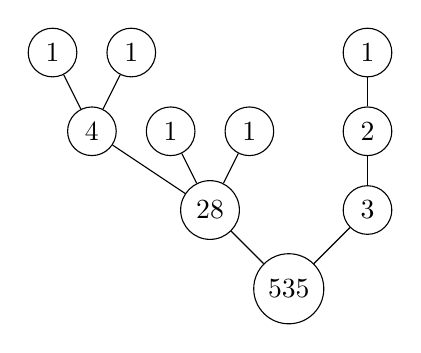
\begin{tikzpicture}
    \node[draw, circle](1_1) at (0,0){1};
    \node[draw, circle](1_2) at (1,0){1};
    \node[draw, circle](1_3) at (4,0){1};
    
    \node[draw, circle](4_1) at (.5,-1){4};
    \node[draw, circle](1_4) at (1.5,-1){1};
    \node[draw, circle](1_5) at (2.5,-1){1};
    \node[draw, circle](2_1) at (4,-1){2};

    \node[draw, circle](28_1) at (2,-2){28};
    \node[draw, circle](3_1) at (4,-2){3};

    \node[draw, circle](535) at (3, -3){535};

    \draw(1_1)--(4_1);
    \draw(1_2)--(4_1);
    \draw(1_3)--(2_1);
    \draw(1_4)--(28_1);
    \draw(1_5)--(28_1);
    \draw(4_1)--(28_1);
    \draw(2_1)--(3_1);
    \draw(28_1)--(535);
    \draw(3_1)--(535);
  \end{tikzpicture}
  \caption{A tree whose vertices are labelled by the corresponding matula numbers. Consider e.g. the node 4, whose predecessors are two nodes labelled 1. Thus, we can compute $4=p(1)\cdot p(1)$. The node labelled 28 can be computed by $28 = p(4)\cdot p(1) \cdot p(1) = 2\cdot 2 \cdot 7$. The node 535 obtains its label by $535=p(28)\cdot p(3) = 107\cdot 5$.}
  \label{fig:matula-illustration}
\end{figure}

While this description could lead to very elegant algorithms in a theoretical setting, it does not come in handy in practice because the matula numbers can be very big (more than 32 bit needed for matula numbers of 15-node intrees).
\end{description}

\section{Enumerating all intrees with a certain number of nodes}
\label{sec:enumerating-all-intrees}

It is clear that the number of intrees (more precisely, the number of unlabelled rooted trees) with exactly $n$ nodes is exponential in $n$ ($1, 1, 2, 4, 9, 20, 48, 115,\dots$ --- see e.g. \cite{flajolet2009analytic} for a derivation of the sequence or refer to \cite{oeisrootedtrees}). However, for experimental purposes, it is convenient to have an algorithm that is capable of enumerating all these intrees. The main thing that should be kept in mind is that we do \emph{not} generate isomorphic intrees over and over again.

We now show an algorithm to generate \emph{all} intrees with a certain number of nodes (called $n$) up to isomorphism. This algorithm is based on the following two facts: 

\begin{itemize}
  \item The overall root can have any amount of children between 1 and $n-1$. If it has only 1 child, the corresponding predecessor intree must contain exactly $n-1$ vertices. If it has exactly $n-1$ children, each predecessor intree contains exactly 1 vertex. All the cases in between admit several possibilities.
  \item If the overall root of the intree with $n$ verices has exactly $r$ predecessors (with $r \in \left\{ 1,2,\dots,n-1 \right\}$, as stated before), then the sum of the vertices with in the predecessor intrees is exactly $n-1$. Moreover, let us denote the predecessor intrees by $T_1,T_2,\dots,T_r$ and call $n_i$ the number of vertices in predecessor intree $T_i$ for all $i\in\left\{1,2,\dots,r \right\}$. Without loss of generality, we can assume $1 \leq n_1 \leq n_2 \leq n_3 \leq \dots \leq n_r$\todo{How many of these \emph{partitions} are there?}.
\end{itemize}

We can exploit these two facts to construct a recursive algorithm which is described in algorithm \ref{alg:generate-intrees}. This algorithm enumerates all intrees with exactly $n$ vertices. It does so by traversing all tuples $(n_1,\dots,n_r)$ fulfilling
\begin{equation*}
  n_1 + n_2 + \dots + n_r = n-1 \quad \text{ and } \quad 1\leq n_1\leq n_2\leq\dots\leq n_r.
\end{equation*}
It then (recursively) generates all combinations of predecessor intrees $(p_1,\dots,p_r)$ whose respective number of nodes are $n_1,\dots,n_r$. The algorithm thereby omits duplicate combinations. This can easily be acchieved by defining an order $\left(\treegeq\right)$ on intrees as follows ($t_1$ and $t_2$ being two intrees with roots $r_1$ resp. $r_2$ and roots' predecessors $p_{1,1}\dots,p_{1,r}$ resp. $p_{2,1},\dots,p_{2,r}$):

\begin{equation}
  \label{eq:definition-treegeq}
  t_1 \treegeq t_2 \equiv (\text{$t_1$ has more vertices than $t_2$}) \vee \exists k \in \left\{ 1,2,\dots,r \right\}. \left( p_{1,k} \treegeq p_{2,k} \wedge \forall i<k. p_{1,i}=p_{2,i} \right)
\end{equation}

\begin{algorithm}
  \begin{algorithmic}[5]
    \Procedure{GenerateIntrees}{$n$} \Comment{Returns the set of all intrees with exactly $n$ vertices}
      \If{$n=1$} 
        \State \textbf{return} $\left\{ \tikz{\fill(0,0) circle (0.1cm);} \right\}$ \Comment{Base case: Intree with just 1 vertex}
      \EndIf
      \State $R \gets \left\{  \right\}$ \Comment{Variable for result}
      \For{$(n_1,\dots,n_r)
            \in 
            \left\{ (n_1,\dots,n_r) \in \naturals^r \mid 
              1 \leq r < n \wedge
              1 \leq n_1 \leq n_2 \leq \dots \leq n_r
            \right\}$}
          \label{alg:huge-for-loop-in-tree-generation}
        \State $P \gets$ (\Call{GenerateIntrees}{$n_1$},\dots,\Call{GenerateIntrees}{$n_r$}) \Comment{Predecessor intrees}
        \For{$(p_1,\dots,p_r) \in P[1] \times P[2] \times \dots \times P[r]$}
          \If{$p_1 \treegeq p_2 \treegeq \dots \treegeq p_r$} \Comment{No duplicates}
          \State $R \gets R \cup \Call{CombinePredecessorIntrees}{p_1,\dots,p_r}$
          \EndIf
        \EndFor
      \EndFor
      \State \textbf{return} $R$
    \EndProcedure
    \Statex
    \Procedure{CombinePredecessorIntrees}{$p_1,\dots,p_r$}
    \State \textbf{return} $\left\{
      \tikz[baseline=(current bounding box.center)]{
        \fill (-0.5,0)circle(0.1cm);
        \node(root) at (-0.5,0){};
        \node[circle](1) at (-2,1) {$p_1$};
        \node[circle](2) at (-1,1) {$p_2$};
        \node[circle](p) at (0,1) {...};
        \node[circle](r) at (1,1) {$p_r$};
        \draw[-] (1) -- (root);
        \draw[-] (2) -- (root);
        \draw[-] (r) -- (root);
      }
      \right\} $
      \Comment{New root with predecessor intrees $p_1,\dots,p_r$}
    \EndProcedure
  \end{algorithmic}
  \caption{Generating all intrees up to isomorphism}
  \label{alg:generate-intrees}
\end{algorithm}

Please note that algorithm \ref{alg:generate-intrees} can be easily adjusted to generate only non-trivial intrees (i.e. intrees whose root has a degree greater than 1) by adding a simple check that shall occur \emph{only in the initial call} of \textsc{GenerateIntrees}: We then simply have to assure that $r$ is greater than 1 in line \ref{alg:huge-for-loop-in-tree-generation}.

Moreover, even if the algorithm is described here in a quite mathematical way, it can be faily easy implemented in e.g. Python. Especially, the ordering of intrees -- that might look complicated at first sight -- can be acchieved with very simplistic methods.

%%% Local Variables:
%%% TeX-master: "../thesis.tex"
%%% End: 